\documentclass[../TGMAFFIRO.tex]{subfiles}

\begin{document}

% Link
As stated in the first chapter, a financial institution selling financial derivatives must take into account certain factors in order to avoid the occurrence of arbitrage against it. One must then inquire about the \textit{correct} price to charge for any of these derivatives. Consider the valuation of the forward seen on chapter 1. Given that a forward is an obligation at a future date, one may price it as the expected value of the asset at maturity, discounted at some rate $r$. Simply put, assuming we can sell many units of a given product, by \textbf{Kolmogorov's Strong Law of Large Numbers (LLN)}, we would expect, in the long run, to break even:

\begin{theorem}
    Let $\{X_n\}_{n\geq 1}$ be a collection of i.i.d. random variables with mean $\mu$. Denote $S_n = \frac{1}{n}\sum_{i=1}^n X_n$. Then, with probability one,
    \begin{equation}
        S_n \to \mu.
    \end{equation}
\end{theorem}

Feasible as this may seem, as pointed out by \aycite{baxter}, this approach could lead to disaster for a financial institution. Let us develop the informal argument about the value of the forward as given in section \ref{sect:risk_hedge_arbitrage}. We first recall that the payoff of a long forward is given by $S - K$. What, then, is the value of $K$ such that no arbitrage is possible?\\

Let us consider a continuously compounded interest rate $r$ and denote $S_t$ the value of the asset at time $t$. At $t=T$, we want $K$ such that the value of the forward is

\begin{equation}\label{eq:forward_future}
  S_T - K = 0.
\end{equation}

A first useful result to compute the present value of the forward is to note that if a payoff has some specified future value, then the present value of the payoff must be the same. That is,
if (\ref{eq:forward_future}) specifies the value of the forward at a future date, then it's price today is the present value of the factors that make the payoff:
\begin{equation}
  S_0 - e^{-rT}K = 0.
\end{equation}

\begin{figure}[hbt]
	\centering
  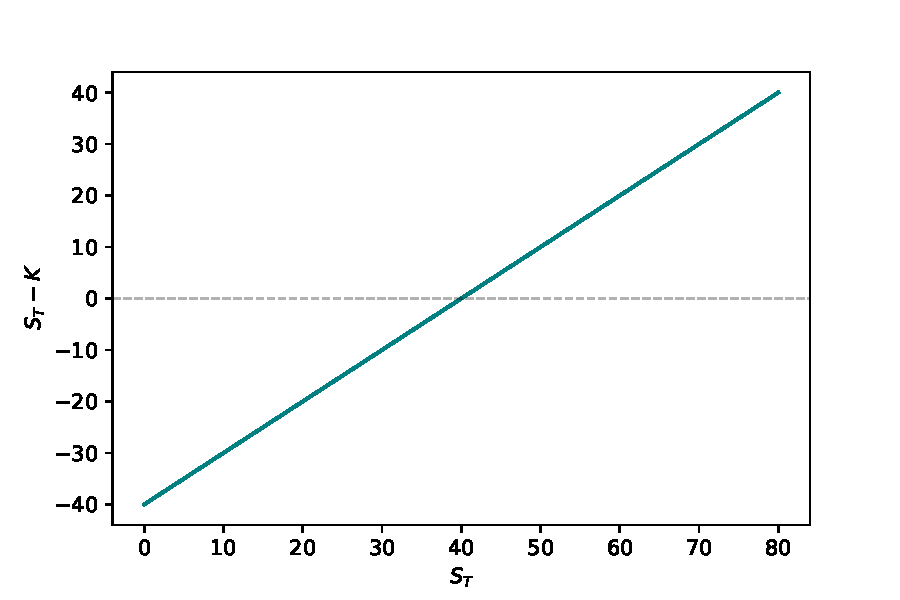
\includegraphics[width=0.7\textwidth]{../images/foward_payoff}
  \caption{Payoff of a forward at maturity.}
\end{figure}

We then conclude that $K=S_0e^{rT}$. To see why, consider any other $K^\prime > K$
\begin{itemize}
	\item at $t=0$, borrow $S_0$; purchase the stock; and take a short position on the forward.
	\item at $t=T$, receive $K^\prime$; deliver the forward; and repay $S_0e^{rT}$. Profit $K^\prime - S_0 e^{rT}$.
\end{itemize}

The same riskless profit can be made if $K^\prime < K$, by taking a long position on the forward.\\


% Focus
With this last example, it is easy to see that the theoretical price anyone should offer for a financial derivative should be such that in which no arbitrage is possible.\\

 In this chapter we aim to develop an intuition behind option valuation for an arbitrage-free price, and hint on what is to expect from a more mathematically-robust model. To achieve the latter we present the binomial-tree model, and relax the mathematical rigor used in the previous chapter.\\

% Overview
We develop this chapter twofold: we first lay the foundations required to value an option using a single binomial tree; the second chapter comprises the generalization of the single binomial tree and we provide an example of its usage.

\section{One-Step Binomial Models}
In order to generalize an arbitrage-free approach to price a European option on a stock, it is desirable to construct a model that truly reflects the market (unlike the LLN approach). In its simplest form, this market should consist of a cash bond and a stock. We will assume, that the market moves in discrete units of time.\\

\textbf{The Stock}\\
Between any two units of time (e.g. from $t=0$ to $t=1$) the stock can either go up with probability $p$, or down with probability $1-p$; it will have an initial value $S_0$; and, with any of these movements, the stock goes up by a factor $u$, or a down by a factor $d$. Evidently, $0 < d < 1 < u$. Finally, we will assume that unlimited amounts of the stock can be bought at any time and there is no cost incurred in the transaction.\\

\begin{figure}[h!]
\centering
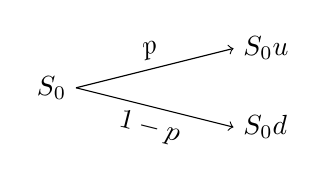
\begin{tikzpicture}
    \draw[->] (0,0) node[left]{$S_0$} --(2, 0.5) node[pos=0.5, sloped, above] {$p$};
    \node[right] at (2, 0.5) {$S_0u$};

    \draw[->] (0,0) --(2, -0.5) node[pos=0.5, sloped, below] {$1-p$};
    \node[right] at (2, -0.5) {$S_0d$};
\end{tikzpicture}
\caption{Possible path of the stock after one unit of time.}
\end{figure}

\textbf{The Bond}\\
The bank account represents the time value of money. We will assume a constant, risk-free, continuously compounding interest rate $r$. For $\$B_0$ invested at $t=0$, said rate guarantees, at the end of $T$ periods, $B_0 e^{rT}$. Also, we will assume that we can lend or borrow at the same interest rate $r$.\\

\textbf{The Derivative}\\
This simple market carries within the possibility of a third that depends on the price of the stock. That is, there could be a payoff with price $f_0$ today that derives its value from the possible directions the stock may take: either $f_u$ if it goes up, or $f_d$ otherwise

\begin{figure}[h!]
\centering
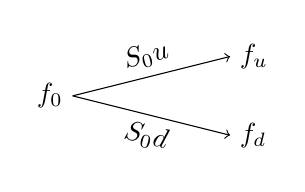
\begin{tikzpicture}
    \draw[->] (0,0) node[left]{$f_0$} --(2, 0.5) node[pos=0.5, sloped, above] {$S_0u$};
    \node[right] at (2, 0.5) {$f_u$};
    \draw[->] (0,0) --(2, -0.5) node[pos=0.5, sloped, below] {$S_0d$};
    \node[right] at (2, -0.5) {$f_d$};
\end{tikzpicture}
\end{figure}


\subsection{Pricing}
We can now ask whether we can construct a portfolio that replicates $f$ from a suitable strategy, thus paying the promised amount. What we are looking for is to guarantee the value of the derivative at the moment of settlement, thus hedging the risk away.\\

Consider the portfolio $(\phi, \psi)$ with $\phi$ number of shares, and $\psi$ monetary units in the bank. At $t=0$, this portfolio is worth

\[
    \phi S_0 + \psi B_0.
\]

At $t=\delta_t$, this portfolio will be worth either $\phi S_0u + \psi B_0e^{r \delta_t}$, or $\phi S_0d + \psi B_0e^{r \delta_t}$.\\

With this in mind, we now turn to answer the initial question. In order to hedge the risk, we would like to find values for $(\phi, \psi)$ in order to replicate the payoff:
\begin{align*}
    \phi S_0u + \psi B_0e^{r \delta_t} = f_u\\
    \phi S_0d + \psi B_0e^{r \delta_t} = f_d
\end{align*}

We can now solve for $\phi$ and $\psi$:

\begin{equation*}
    \phi S_0(u - d) = f_u - f_d.\\
\end{equation*}

\begin{equation} \label{eq:phi}
    \phi = \frac{f_u - f_d}{S_0(u-d)}.
\end{equation}

\begin{align*}
    \psi &= e^{-r\delta_t} [f_u - \phi u]\\
         &= e^{-r\delta_t} \left[f_u - \frac{f_u - f_d}{S_0(u - d)} S_0u\right]\\
         &= e^{-r\delta_t} \frac{uf_d - df_u}{u -d}.
\end{align*}

Thus, buying the portfolio $(\phi, \psi)$ guarantees the payoff at $t=\delta_t$. Denote $\mathcal{V}$ the value of the portfolio at $t=0$. The value of $\mathcal{V}$ is:

\begin{align*}
    \mathcal{V} &= \phi S_0 + \psi\\
                &= \left[\frac{f_u - f_d}{S_0(u - d)}S_0\right] + \left[e^{-r\delta_t}\right]\\
                &= e^{-r\delta_t}\left[\frac{e^{r\delta_t}(f_u - f_d + uf_d - df_u)}{u - d}\right]\\
                &= e^{-r\delta_t}\left[\frac{e^{r\delta_t}f_u - df_u}{u-d} + \frac{uf_d - e^{r\delta_t}f_d}{u-d}\right].
\end{align*}

Therefore,
\begin{equation} \label{eq:v_price_complete}
	\mathcal{V} = e^{-r\delta_t}\left[f_u \frac{e^{r\delta_t} - d}{u - d} + f_d \frac{u - e^{r\delta_t}}{u-d}\right].
\end{equation}

$\mathcal{V}$ is the cost of a risk-free strategy that guarantees the payoff, and assures the impossibility to commit arbitrage. Consider any other price $\mathcal{P} < \mathcal{V}$. Buying the portfolio $\mathcal{P}$ and selling $\mathcal{V}$ at $t=0$ guarantees, at $t=\delta_t$, enough money to settle and earn $\mathcal{V}-\mathcal{P}$ risk-free. The same argument can be done for a value $\mathcal{P} > \mathcal{V}$.\\

What, then, would have happened, had we decided to replicate this payoff using only the bank account and the probabilities $p$ and $1-p$? Accordingly, we would've priced the derivative at the present value of the expected payoff under the $\mathbb{P}$ measure. Denote $\hat{\mathcal{V}}$ this alternate value, then:

\begin{equation}
    \hat{\mathcal{V}} = \exp(-r\delta_t)\mathbb{E}[f] = \exp(-r\delta_t)[f_u \cdot p + f_d \cdot (1- p) ].
\end{equation}


Pricing $\hat{\mathcal{V}}$ for $f$ does not guarantee $\hat{\mathcal{V}} = \mathcal{V}$, which could lead to arbitrage otherwise. Assuming $\hat{\mathcal{V}} \neq \mathcal{V}$, the expected payoff of $f$ would not be $\hat{\mathcal{V}}$, market participants would be inclined to make a profit, thereby breaking the assumption that every position taken on the derivative is independent of one another; we cannot expect to break even in the long run.


%TODO: Explain more about the Q-measure
\subsection{The Q Measure}
Consider  (\ref{eq:v_price_complete}) with payoff $S_T - K$ (a long forward).

\begin{equation*}
    \mathcal{V} = e^{-r\delta_t}\left[S_0u \frac{e^{r\delta_t} - d}{u - d} + S_0d \frac{u - e^{r\delta_t}}{u-d}\right].
\end{equation*}

Denote
\begin{equation}
    q:= \frac{\exp{r\delta_t} - d}{u - d} \Longrightarrow 1-q = \frac{u - \exp{(r\delta_t)}}{u-d}.
\end{equation}\\

We can argue that $d < \exp{(r\delta_t)} < u$ implies no arbitrage. To see why, 
\begin{enumerate}
\item Suppose $\exp{(r\delta_t)} < d < u$.\\
    At t=0 we can borrow $\$S_0$ and buy the stock. At $t=\delta_t$, we collect either $S_0u$ or $S_0d$, thereby making a risk-free profit of $S_0(u - \exp{(r\delta_t)})$ or $S_0(d - \exp{(r\delta_t)})$.

\item Suppose $d < u < \exp{(r\delta_t)}$\\
    At $t=0$, lend $\$S_0$ and short the stock. At $t=\delta_t$, collect $S_0\exp{(r\delta_t)}$ and buy the stock at either $S_0u$ or $S_0d$. Again, this guarantees a risk-free profit of either $S_0(\exp{(r\delta_t)} - u)$ or $S_0(\exp{(r\delta_t)} - d)$.
\end{enumerate}

Being $d < \exp{(r\delta_t)} < u$ implies $0 < q < 1$. We can rewrite \ref{eq:v_price_complete} as
\begin{equation} \label{eq:v_price}
    \mathcal{V} = \exp{(-r\delta_t)}[S_0u\cdot q + S_0d \cdot (1-q)].
\end{equation}


$\mathcal V$ is the discounted expectation under a probability measure $\mathbb Q$; it is not the expected value of the derivative, but a change in the measure of the tree such that guarantees no arbitrage. Theoretically, this is backed up by the Radon-Nikodym derivative (see theorem \ref{th:radon-nikodym}).

\section{Generalized Binomial Tree Model}
In order to generalize our model to $n$ periods we only need to consider each node as the root of another binomial tree. Consequently, we get a tree with $n$ periods and $2^n$ nodes at $t=n$.\\

\begin{figure}
\centering
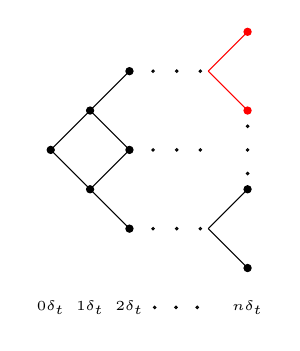
\begin{tikzpicture}
    % First Node
    \draw[-] (0,0) -- (0.5, 0.5);
    \draw[-] (0,0) -- (0.5, -0.5);
    \draw[black, fill=black](0.5,-0.5) circle (.3ex);
    \draw[black, fill=black](0.5,0.5) circle (.3ex); 
    \draw[black, fill=black](0,0) circle (.3ex);

    % 1) up node
    \draw[-](0.5, 0.5) -- (1, 1);
    \draw[-](0.5, 0.5) -- (1, 0);
    \draw[fill=black] (1,1) circle (.3ex);
    \draw[fill=black] (1,0) circle (.3ex);
    % 1) down node 
    \draw[-](0.5, -0.5) -- (1, 0);
    \draw[-](0.5, -0.5) -- (1, -1);
    \draw[fill=black] (1,-1) circle (.3ex);
    
    % Connection points
    \draw[black](1.3, 1) circle (.1ex);
    \draw[black](1.6, 1) circle (.1ex);
    \draw[black](1.9, 1) circle (.1ex);

    \draw[black](1.3, 0) circle (.1ex);
    \draw[black](1.6, 0) circle (.1ex);
    \draw[black](1.9, 0) circle (.1ex);


    \draw[black](1.3, -1) circle (.1ex);
    \draw[black](1.6, -1) circle (.1ex);
    \draw[black](1.9, -1) circle (.1ex);
    
    \draw[black](2.5, 0.3) circle (.1ex);
    \draw[black](2.5, 0) circle (.1ex);
    \draw[black](2.5, -0.3) circle (.1ex);

    % 2.1) up node
    \draw[-, red](2, 1) -- (2.5, 1.5);
    \draw[-, red](2, 1) -- (2.5, 0.5);
    \draw[red, fill=red] (2.5, 1.5) circle (.3ex);
    \draw[red, fill=red] (2.5,0.5) circle (.3ex);
    % 2.2) down node 
    \draw[-](2, -1) -- (2.5, -0.5);
    \draw[-](2, -1) -- (2.5, -1.5);
    \draw[fill=black] (2.5,-0.5) circle (.3ex);
    \draw[fill=black] (2.5,-1.5) circle (.3ex);

    \node[font=\fontsize{4}{4}] at (0, -2) {$0\delta_t$};
    \node[font=\fontsize{4}{4}] at (0.5, -2) {$1\delta_t$};
    \node[font=\fontsize{4}{4}] at (1, -2) {$2\delta_t$};
    \draw (1.32, -2) circle (.1ex);
    \draw (1.59, -2) circle (.1ex);
    \draw (1.86, -2) circle (.1ex);
    \node[font=\fontsize{4}{4}] at (2.5, -2) {$n\delta_t$};
\end{tikzpicture}
\caption{The $n$-period model}
\end{figure}

To motivate this generalized model, we will now present an example of a $3$-period binomial model.
% Find another name for this example..
\subsection{An Example}
Suppose that at $t=0$ we have a stock worth $S_0=100$ that can go up by a factor of $1.20$, or down by a factor of $0.80$. Assume further that the $\mathbb{P}$ measure probability for an up move is $\frac{3}{4}$, finally, suppose $r=0$. Being consistent with the notation used, $u=1.20$, $d=0.80$, $p = \frac{3}{4}$ and $ 1 - p = \frac{1}{4}$.\\

We set up to price a call option on $S_0$ with strike price $K=110$, three periods from now. Denote $f_t$ the value of the derivative at time $t$. The payoff at maturity ($t=3$) is

\begin{equation}
    f_3 = \max\{S_3 - K, 0\} =: [S_3 - K]^+.
\end{equation}

Since $S$ can either move up or down with known factors $u$ and $d$ respectively, we know all the values the stock can take up to $t=3$. For example, from $t=0$ to $t=1$, the stock can either move to $100 \cdot 1.20$, or down to $100 \cdot 0.80$.\\

\begin{figure}
\centering
\begin{tikzpicture}
    \node (s) at (0,0) {100};

    \node[above right = 0.5cm of s] (su) {120}; \draw[->] (s) -- (su);
    \node[below right = 0.5cm of s] (sd) {80};  \draw[->] (s) -- (sd);

    \node[above right = 0.5cm of su] (suu) {144}; \draw[->] (su) -- (suu);
    \node[below right = 0.5cm of su] (sud) { 96}; \draw[->] (su) -- (sud); \draw[->] (sd) -- (sud);
    \node[below right = 0.5cm of sd] (sdd) { 64}; \draw[->] (sd) -- (sdd);

    \node[above right = 0.5cm of suu] (suuu) {172.8}; \draw[->] (suu) -- (suuu);
    \node[below right = 0.5cm of suu] (suud) {115.2}; \draw[->] (suu) -- (suud); \draw[->] (sud) -- (suud);
    \node[below right = 0.5cm of sud] (sudd) { 76.8}; \draw[->] (sud) -- (sudd); \draw[->] (sdd) -- (sudd);
    \node[below right = 0.5cm of sdd] (sddd) { 51.2}; \draw[->] (sdd) -- (sddd);
\end{tikzpicture}
\caption{The Stock Process}
\end{figure}

Given $f$ and the stock-tree process we can compute, for example, the amount to be paid if the stock moves up at every step. Under this scenario, $S_3 = 172.8$. Then $f(S_3) = [172.8 - 110]^+ = 62.80$, which means that the buyer of the option would receive $\$62.80$. Computing the payoff at every last node yields a set of payoffs at maturity.\\

With the set of payoffs at maturity, we proceed to find the value of the option at every other node in the tree solving iteratively from $t=2$ to $t=0$.\\

For example, the upper node at $t=2$ is computed by taking the discounted expectation under the $\mathbb{Q}$ measure as shown in \ref{eq:v_price}. Were the stock to climb up two times then, the payoff at $t=3$ can either be 62.8 or 5.2. Denote $f^{uu}_2$ the value the derivative at $t=2$ for the upper node, its value is then

\begin{equation*}
    f^{uu}_2 = \exp(-0)[62.8q + 5.2(1-q)] = 34; \  q = \frac{0 - 0.80}{1.20 - 0.80}.
\end{equation*}\\

\begin{figure}
\centering
\begin{tikzpicture}
    \node (s) at (0,0) {10.45};

    \node[above right = 0.5cm of s] (su) {18.3}; \draw[->] (s) -- (su);
    \node[below right = 0.5cm of s] (sd) {2.60};  \draw[->] (s) -- (sd);

    \node[red, above right = 0.5cm of su] (suu) {34}; \draw[->] (su) -- (suu);
    \node[below right = 0.5cm of su] (sud) {2.60}; \draw[->] (su) -- (sud); \draw[->] (sd) -- (sud);
    \node[below right = 0.5cm of sd] (sdd) {0.00}; \draw[->] (sd) -- (sdd);

    \node[above right = 0.5cm of suu] (suuu) {62.8}; \draw[->] (suu) -- (suuu);
    \node[below right = 0.5cm of suu] (suud) {5.20}; \draw[->] (suu) -- (suud); \draw[->] (sud) -- (suud);
    \node[below right = 0.5cm of sud] (sudd) {0.00}; \draw[->] (sud) -- (sudd); \draw[->] (sdd) -- (sudd);
    \node[below right = 0.5cm of sdd] (sddd) {0.00}; \draw[->] (sdd) -- (sddd);

    \draw[red, dashed] (2,0.65) -- (4.1,0.65) -- (4.1, 2.8) -- (2, 2.8) -- (2, 0.65);
    \end{tikzpicture}
\caption{The Claim Tree}
\end{figure}

Loosely speaking, every node in the claim-tree represents the value of the option at every step. Evidently, at $t=3$, the value of the option can only be its current value since there is nowhere to move elsewhere in the tree. At $t=0$ we have the risk-free value for the option that guarantees no arbitrage.\\

% TODO: Add definition of self-financing portfolio
To see why this is true, suppose we were to sell this option at \$10.45. For the sake of the argument, suppose the stock moves up two times and down at the last time-tick. If 10.45 is truly the arbitrage-free price option, we should be able to replicate the movement of the stock at each time interval and arrive at the payoff without incurring any other cost.\\

According to equation \ref{eq:phi}, at $t=0$ we would need to buy 0.3925 units of $S$ and borrow 28.8 to cover the expenses; if the price goes up at $t=1$, around 0.65 units of the stock are required, which would lead to a purchase of 0.26 extra units of the stock, thus incrementing the amount borrowed to 60.2. At $t=2$, 1 unit of $S$ is required, increasing the amount borrowed to 110. Finally, at $t=3$, the stock takes a down move and \$5.2 is the amount owed to the option buyer. \\

The final value in the position of the stock is $S_0 u ^ 2 d \cdot \phi = 115.20$, minus the \$110 owed, brings the total value of the portfolio to \$5.20, exacltly the amount required to fulfill the obligation.
\end{document}
